% pdflatex -shell-escape template_cdc.tex

\documentclass[a4paper,oneside]{article}

\usepackage[frenchb]{babel}
\usepackage[utf8]{inputenc}
\usepackage[T1]{fontenc}
\usepackage{graphicx}
\usepackage{amssymb} 
\usepackage{amsmath}
\usepackage{hyperref}
\usepackage{fullpage}
\usepackage{epstopdf}


%%%%%%%%%%%%%%%%%%%%%%%%%

\newcommand{\mytitle}{Projet Gloup - Cahier des charges}
\title{\mytitle } 

%%%%%%%%%%%%%%%%%%%%%%%%%

\makeatletter

\usepackage{fancyhdr}
\pagestyle{fancyplain}
\fancyhf{}
\renewcommand{\headrulewidth}{0pt}
\renewcommand{\footrulewidth}{0.5pt}
\lfoot{\mytitle}
\cfoot{\@date}
\rfoot{page \thepage / \pageref{fin}}

\author{Ginette et Roger}

\date{1\ier~juin 2015}


%%%%%%%%%%%%%%%%%%%%%%%%%


\begin{document}

\maketitle

\thispagestyle{fancyplain}


%%%%%%%%%%%%%%%%%%%%%%%%%

\section{Renseignements}

\paragraph{Nom du projet :}
Gloup

\paragraph{Objet :}
Développement d'un logiciel de gestion d'un stock de bières sur grille-pain

\paragraph{Maître d'ouvrage :}
Ginette

\paragraph{Maître d'oeuvre : }
Roger

\paragraph{Date de début :}
1\ier~juin 2015

\paragraph{Date de fin :}
18 juin 2015


%%%%%%%%%%%%%%%%%%%%%%%%%

\newpage

\section{Définition du besoin}

\paragraph{Contexte général\\}
Au fond de sa cuisine, Ginette entrepose le stock de bière dans une cave électronique thermo-régulée.
Malheureusement, comme ce stock est utilisé de façon assez intensive, il est difficile d'assurer son approvisionnement.
Ginette a donc besoin d'un logiciel pour gérer ce stock efficacement.
Heureuse coïncidence, il y a un grille-pain Gogol-Connected à écran tactile posé sur la cave électronique et Ginette a réussi à le jailbreaker pour y installer un système NetBSD pouvant accueillir le logiciel de gestion de stock à développer.


\paragraph{Besoins et priorités\\}
Le besoin principal est de pouvoir gérer le stock : entrer/sortir des bières, faire l'inventaire du stock...
L'interface doit être simple et efficace, pour que le logiciel reste exploitable par d'autres personnes ou lors des "coups de feux".
Enfin, il serait intéressant de pouvoir réapprovisionner le stock depuis le logiciel, via le webservice du fournisseur.


%%%%%%%%%%%%%%%%%%%%%%%%%

\newpage

\section{Spécifications}

\begin{itemize}
    \item logiciel fonctionnant sur les grilles-pains "Flash Gordon Toaster II" à système NetBSD
    \item fonctionnalités de gestion du stock de bières :
        \begin{itemize}
            \item entrer des bières dans le stock
            \item sortir des bières du stock
            \item afficher l'inventaire du stock 
            \item paramétrer les types de bières possibles
        \end{itemize}
    \item interface utilisateur :
        \begin{itemize}
            \item interface graphique pour écran tactile de résolution $1080 \times 1920$
            \item affichage simple avec zones tactiles d'au moins $100 \times 100$ pixels
        \end{itemize}
    \item performances demandées :
        \begin{itemize}
            \item gestion d'au moins 20 types de bières avec au moins 10 bouteilles de chaque type
            \item temps de réponse des actions inférieurs à 100 ms 
        \end{itemize}
    \item fonctionnalités de réapprovisionnement :
        \begin{itemize}
            \item accès au webservice par protocole BSTP (Beer Supply Transport Protocol) RFC 1664 avec confirmation différée par appel téléphonique du fournisseur
            \item page dédiée dans l'interface utilisateur : 
                \begin{itemize}
                    \item sélection des types de bière et quantités 
                    \item sélection de la durée minimale avant confirmation téléphonique (0, 15 min, 30 min ou 1 h)
                \end{itemize}
        \end{itemize}
\end{itemize}


%%%%%%%%%%%%%%%%%%%%%%%%%

\newpage

\appendix

\section{Livrables}

\begin{itemize}
    \item logiciel déployé sur le grille-pain de Ginette
    \item code source documenté sous licence WTFPL v2 
    \item manuel d'installation et de configuration
    \item manuel d'utilisation
\end{itemize}

\section{Diagrammes de cas d'utilisation}

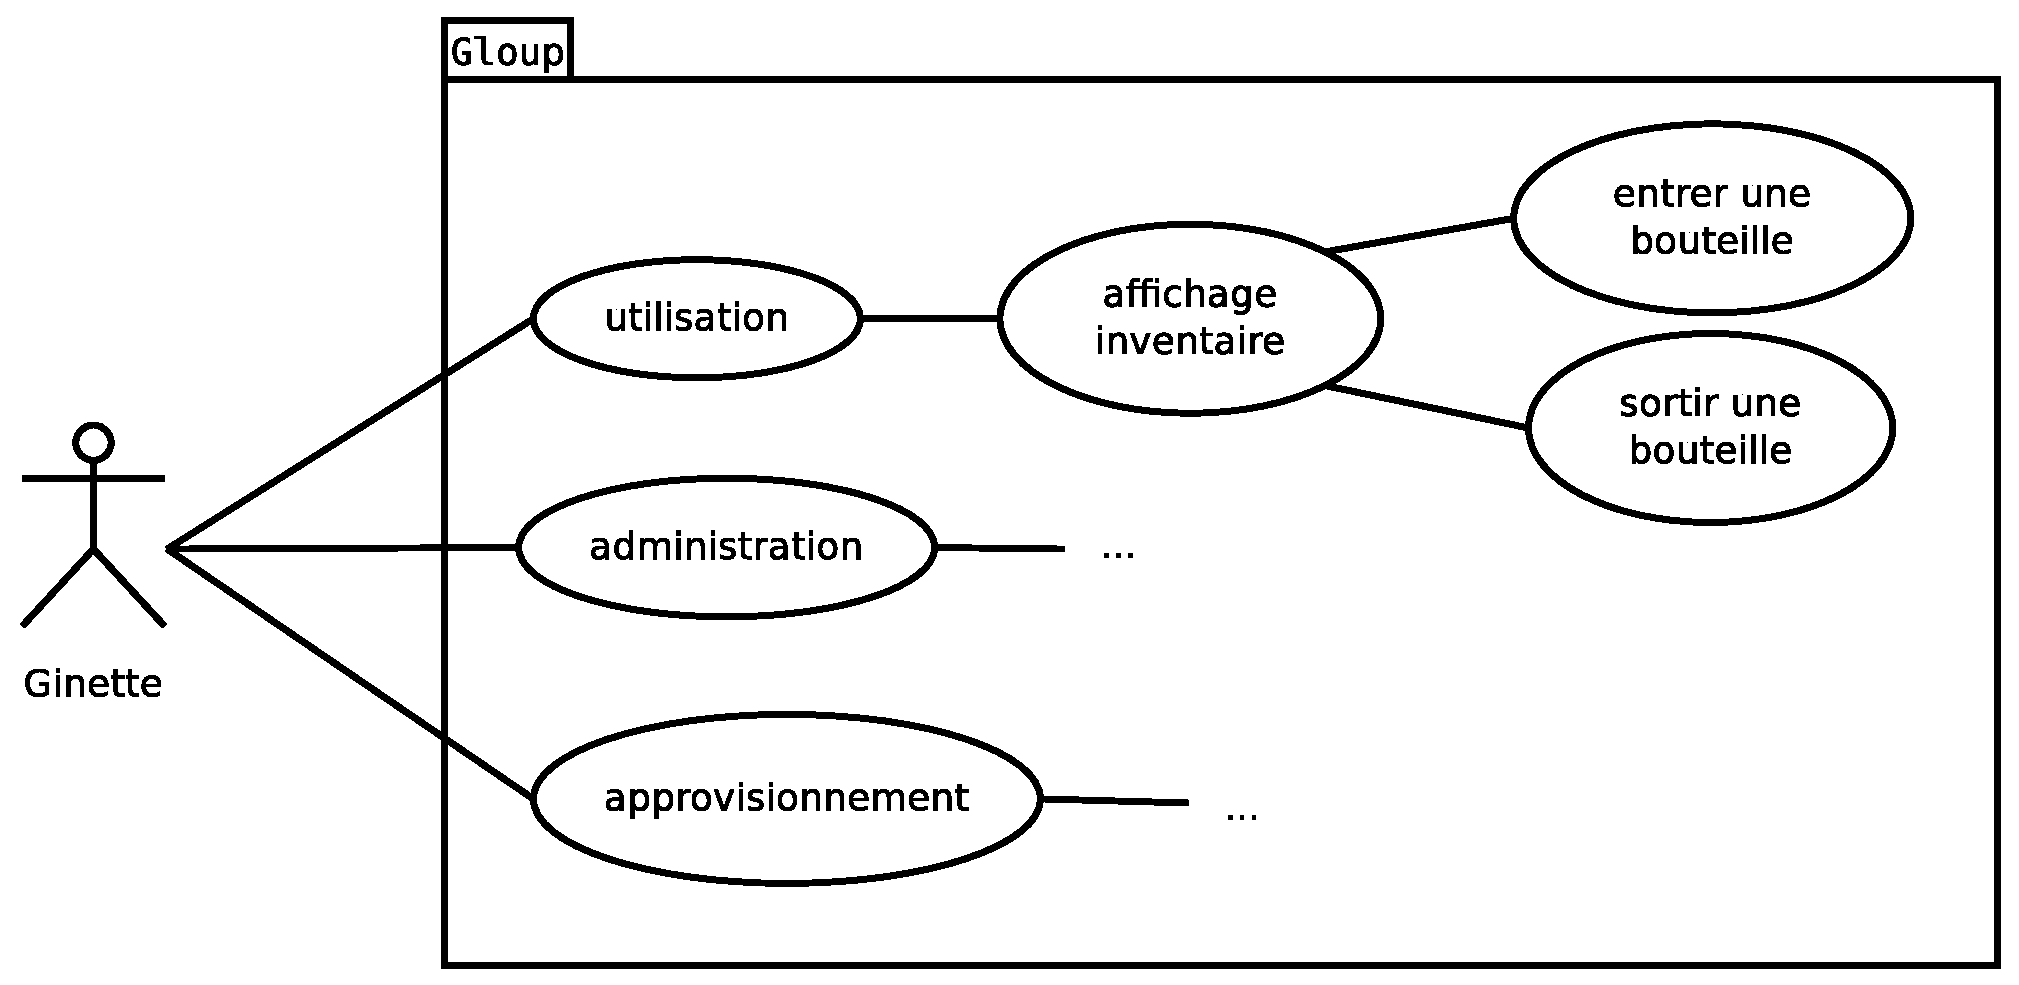
\includegraphics[width=11cm]{cdc_use_case.eps}




\section{Maquettes}

\paragraph{Page utilisation}

~\\


\includegraphics[width=9cm]{cdc_maquette1.eps}

\paragraph{Page administration\\}

...

\paragraph{Page approvisionnement\\}

...





\section{Planning prévisionnel}

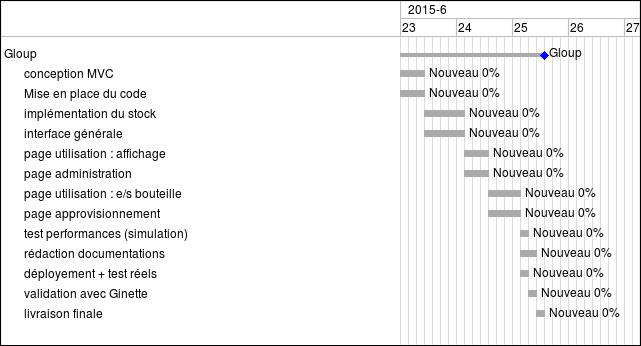
\includegraphics[width=13cm]{cdc_gantt.png}


\section{...}


%%%%%%%%%%%%%%%%%%%%%%%%%

\label{fin}

\end{document}


